\documentclass[10pt,aspectratio=169]{beamer}

\usetheme[progressbar=frametitle]{metropolis}

\title{Mathematical Foundations of Computer Science}
\subtitle{Decidability of string graphs}
\date{19.11.2021}
\author{Pavel Zwerschke}
\institute{Radboud University Nijmegen}
\titlegraphic{\hfill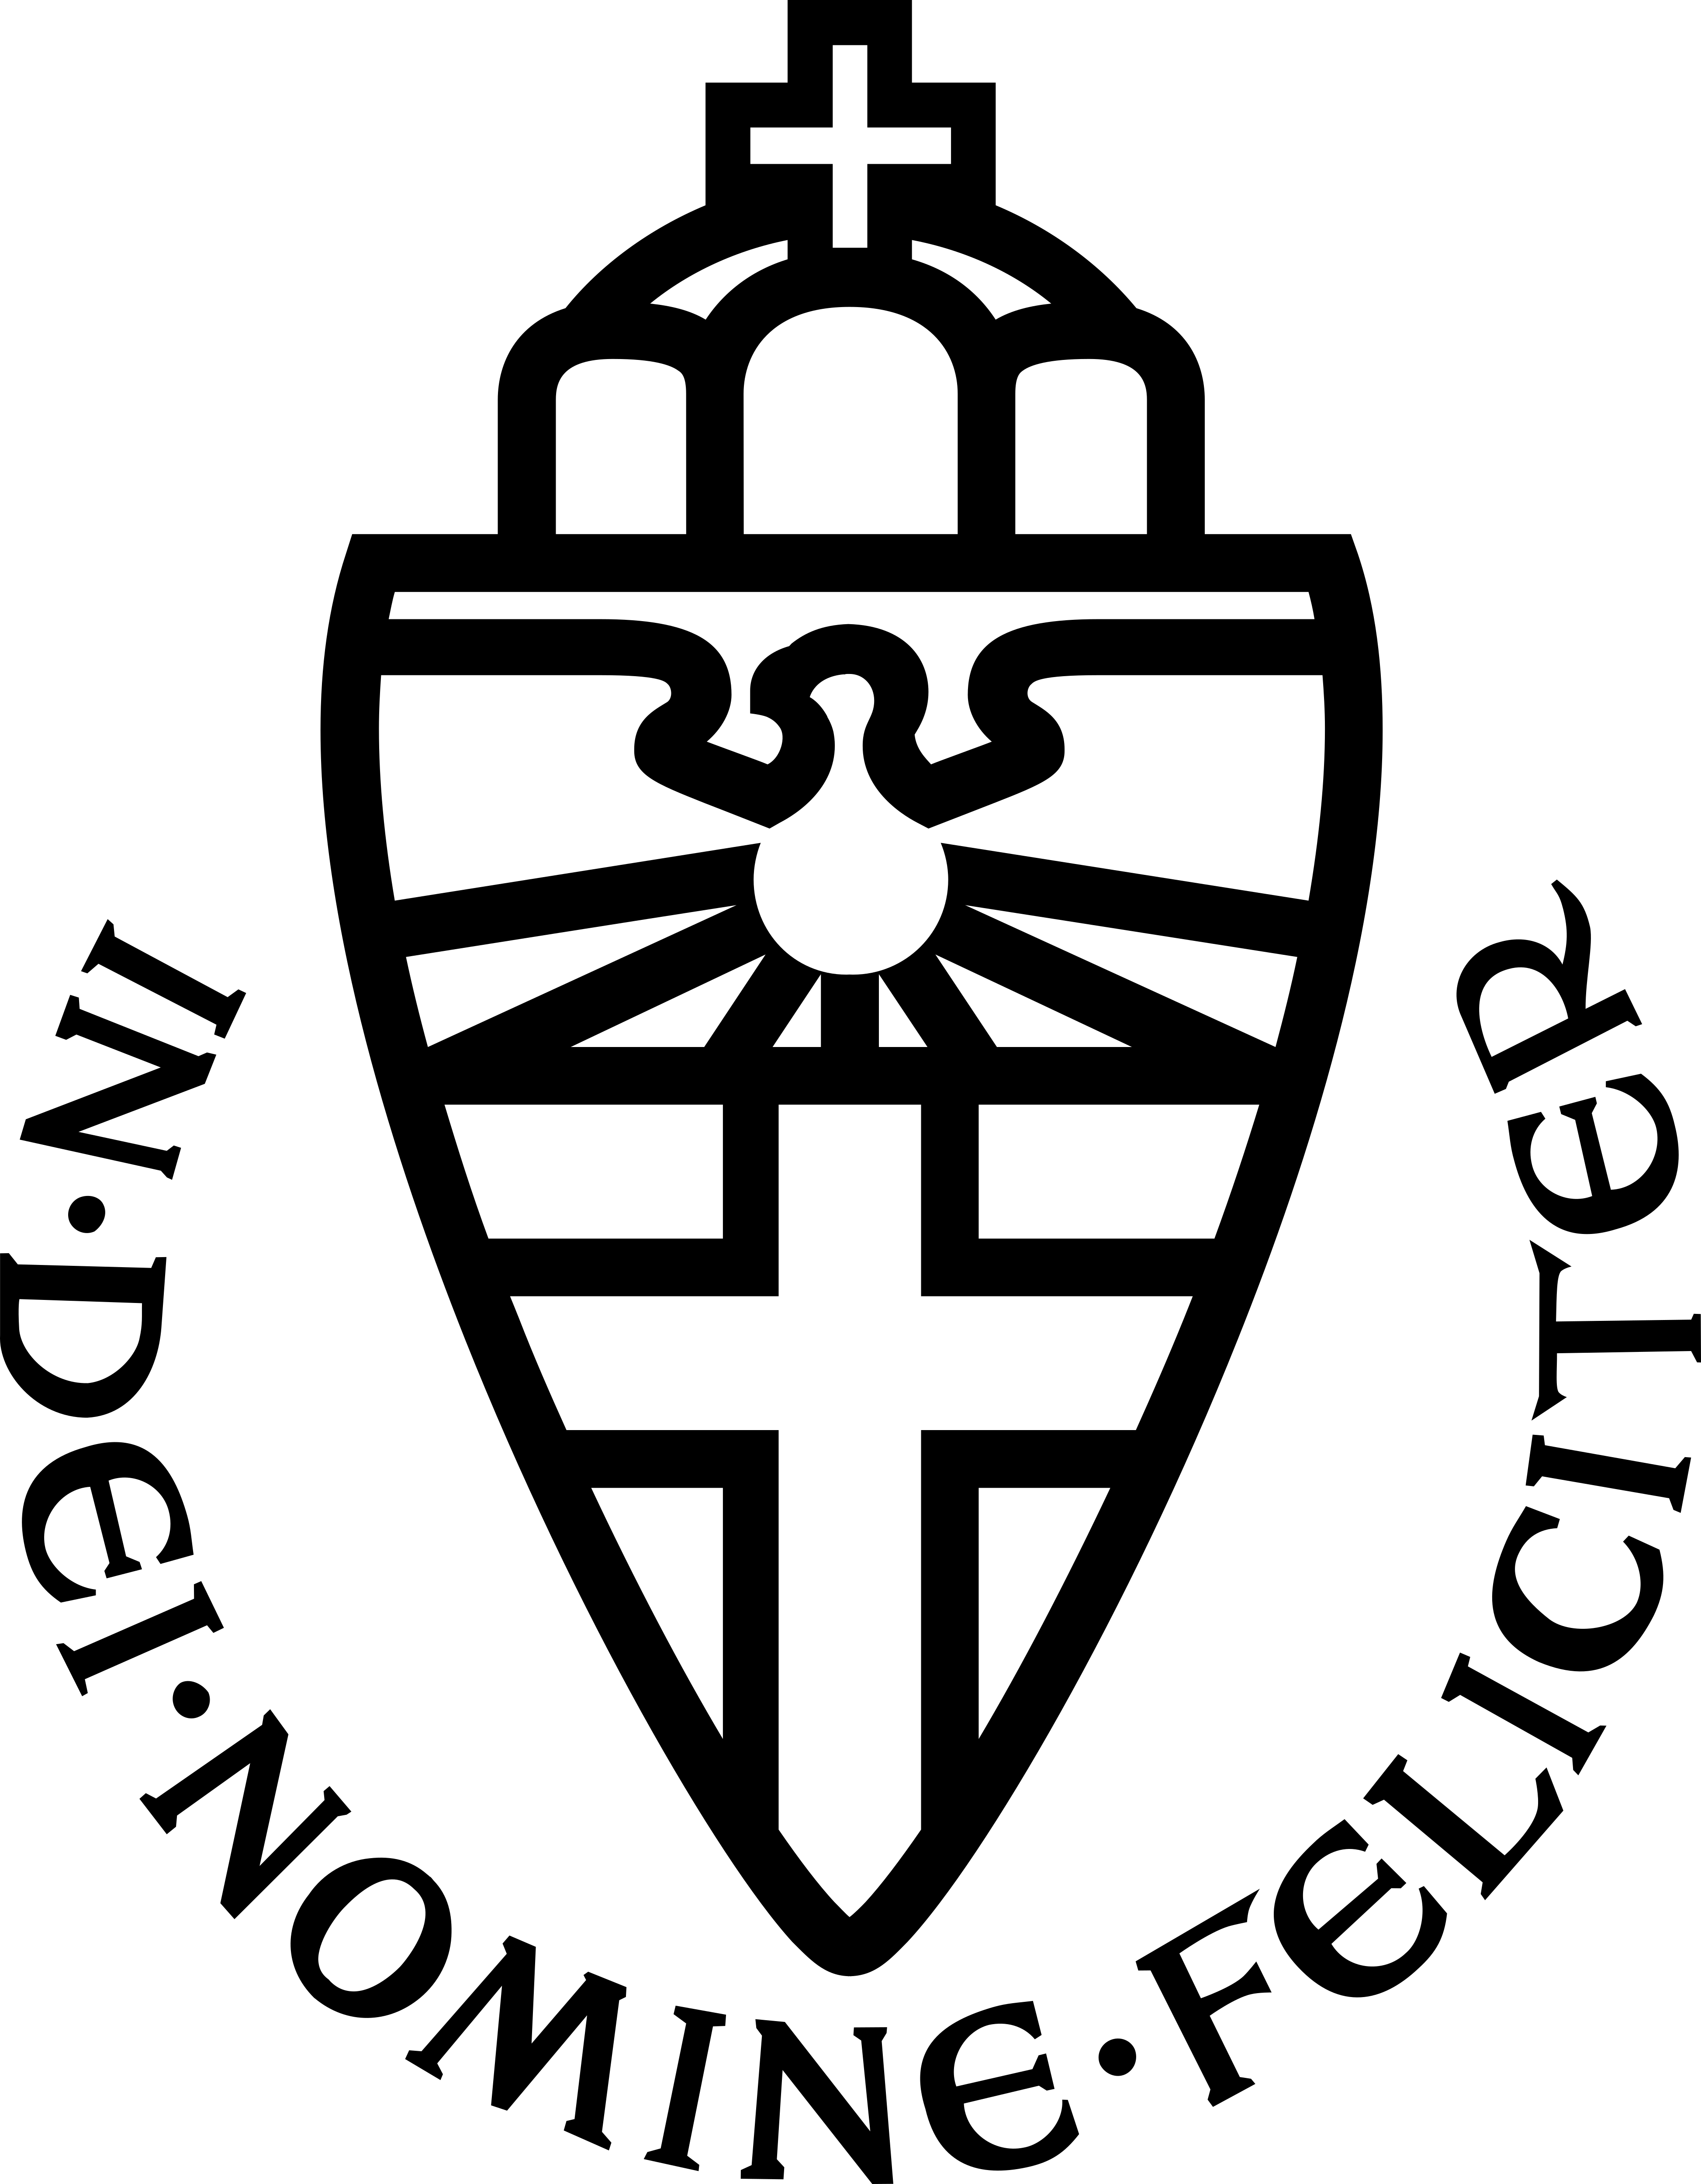
\includegraphics[height=1.5cm]{logos/radboud-university}}

% BibTeX setup
\usepackage[backend=bibtex, bibstyle=alphabetic, citestyle=alphabetic]{biblatex}
\bibliography{references}

\usepackage[english]{babel} % English

% Standard packages for math-related things.
\usepackage{amsmath}
\usepackage{amssymb}
\usepackage{amsthm}
\usepackage{mathtools}

\usepackage{graphicx} % to include graphics with \includegraphics[options]{imagefile}

\theoremstyle{plain} % Usual style for theorems, etc.

\setbeamertemplate{theorems}[numbered]

\theoremstyle{remark} % Usual style definitions.
\newtheorem{remark}[theorem]{Remark}

\newcommand{\N}{\mathbb{N}}
\newcommand{\R}{\mathbb{R}}
\newcommand{\Z}{\mathbb{Z}}

\newcommand{\set}[1]{\{#1\}}
\newcommand{\norm}[1]{\|#1\|}

\begin{document}

\maketitle

\begin{frame}{Table of contents}
    \setbeamertemplate{section in toc}[sections numbered]
    \tableofcontents%[hideallsubsections]
\end{frame}

\section{Introduction}

\begin{frame}{What is a string graph?}
    \begin{itemize}
        \item A \textit{curve} (or \textit{string}) is a set homeomorphic to \([0,1]\)
        \item Given a collection of curves \((C_i)_{i \in I}\) in the plane, the corresponding intersection graph is \( (I, \set{\set{i, j} : C_i \text{ and } C_j \text{ intersect}}) \)
        \item \textit{string graph}: a graph isomorphic to the intersection graph of a collection of curves 
    \end{itemize}
\end{frame}

\begin{frame}{Definitions}
    \begin{itemize}
        \item \textit{size} of a collection of curves: the number of intersection points
        \item Let \(c_s(G)\) be the size of the smallest (smallest number of intersections) set of curves whose intersection graph is isomorphic to \(G\)
        \item Define \(c_s(m) = \max\set{c_s(G) : G \text{ has } m \text{ edges}}\)
    \end{itemize}
\end{frame}

\begin{frame}{\(c_s(G)\) is finite}
    \begin{itemize}
        \item It is not obvious that \(c_s(G)\) is finite for every string graph \(G\)
        \item Kratochvíl et al. showed that \(c_s(G)\) is finite for every string graph \(G\)
    \end{itemize}
    \begin{lemma}
        A string graph can be realized by a family of polygonal arcs with a finite number of intersections.
    \end{lemma}
\end{frame}

\begin{frame}{Realizability}
    \begin{itemize}
        \item Graph \(G = (V, E)\), \(R \subseteq \binom{E}{2} = \set{\set{e, f} : e, f \in E} \) on \(E\)
        \item call a drawing \(D\) of \(G\) in the plane a \textit{weak realization} of \((G, R)\) if only pairs of edges which are in \(R\) are allowed to intersect in \(D\)
        \item call a drawing \(D\) of \(G\) in the plane a \textit{realization} of \((G, R)\) if exactly pairs of edges which are in \(R\) are intersect in \(D\)
        \item \(c_w(G, R)\) is the smallest number of intersections in a weak realization of \((G, R)\)
        \item \(c_w(G) = \max\set{c_w(G, R) : (G, R) \text{ has a weak realization}} \)
        \item \(c_w(m) = \max\set{c_w(G) : G \text{ has } m \text{ edges}}\)
        \item Define \(c_r(G, R)\), \(c_r(G)\) and \(c_r(m)\) similarly for realizations
        \item \(\mathrm{cr}(G) = c_w(G, \binom{E}{2})\) is known as the crossing number (\textbf{NP}-complete)
        \item \(c_w(G, \emptyset)\) is equivalent to planarity testing (in \textbf{P})
    \end{itemize}
\end{frame}

\begin{frame}{Relationships between realizability functions}
    \begin{lemma}
        \begin{enumerate}
            \item \(c_w(m) \leq c_r(m)\)
            \item \( c_r(m) \leq 4 c_s(m^2 + 4m) \)
            \item \(c_s(m) \leq 4 c_w(2m) + 2m\)
        \end{enumerate}
    \end{lemma}
\end{frame}

\section{Bounding the Number of Intersections}

\begin{frame}{Bounding the Number of Intersections 1}
    Assign each curve a unique number \(\leadsto\) intersections along a particular curve is a word over an alphabet
    \begin{lemma}
        Every word of length \(\geq 2^n\) over an alphabet of size \(n\) contains a non-trivial subword in which every character occurs an even number of times.
    \end{lemma}
\end{frame}

\begin{frame}{Bounding the Number of Intersections 2}
    \begin{theorem}
        Let \(G\) be a graph with \(m\) edges, \(R \subseteq \binom{E}{2}\) such that \((G, R)\) is weakly realizable, and let \(D\) 
        be a weak realization of \((G, R)\) with the minimal number of intersections. Then for any edge \(e \in G\) 
        there are less than \(2^m\) intersections on the curve realizing \(e\) in \(D\).
    \end{theorem}
    \begin{corollary}
        String graph recognition is in \textbf{NEXP}.
    \end{corollary}
\end{frame}

\section{String Graphs Requiring Exponential Representations}

\begin{frame}{String Graphs Requiring Exponential Representations}
    Goal: provide a construction of a graph on \(O(n)\) vertices which can be represented as the intersection graph 
    of a system of curves in the plane but every realization of the graph requires an exponential number of intersections.
\end{frame}

\section{Topological Inference}

\begin{frame}{TODO}
    
\end{frame}

\end{document}
